\chapter{Load Generating Tool}
Performance and load testing has been conducted ever since applications came into been. There is a sea of different tools that can fulfill the task of generating virtual end users. In the case of this thesis, the server's capacity is going to be driven to its limit, after which instead of staying overloaded, it will try to scale and consume more clients. This requires the testing tool to be capable of generating a large enough amount of end users. 

\section{JMeter}
\\One of the most popular testing tools is JMeter which is based on Java and cross-platform. It supports multiple protocol and has a very friendly UI to configure test plans. It even produces aggregated test results in different type of graphs. It seems JMeter has everything one asks for except scalibility. When the test requires a bigger scale, JMeter client machine quickly runs into issue that it is unable, performance-wise, to simulate enough users to stress the server or is limited at network level. An option to work around this performance limitation is to utilize remote/distributed testing \citep{JMeterRemote}to control multiple remote JMeter engines from a single JMeter client. In this way, one can replicate a test across many low-end computers and thus simulate a larger load on the server. However, remote mode does use more resources than running the same number of non-GUI tests independently. If many server instances are used, the client JMeter can become overloaded, as can the client network connection. Another inconvenience of using JMeter is to find a ideal environment to host it. While one can execute the JMeter engine on the application server, one can not ignore the fact that this will be adding processing overhead on the application server, consequently  the testing results will be somewhat tainted. All put together, it is decided not to use JMeter as load generating and testing tool in the thesis. \\

\section{nGrinder}
nGrinder \citep{NGrinder} is a platform for stress tests that enables you to execute script creation, test execution, monitoring, and result report generator simultaneously. nGrinder consists of two major components. One is  controller, a web application that enables the performance tester to create a test script and configure a test run. One is agent, a virtual user generator that creates loads. 
The performance team of Cloud Foundry in SAP has conducted their load test on router with nGrinder. The controller operates in a dedicated AWS c3.xlarge instance with 4 CPUs and 7.5 GB memory. Four agents are installed to create loads. Two of those agents are running on the host machine with controller and two others are distributed to another AWS c3.xlarge virtual machine. It manages to produce a load of 8500 requests per second to be handled by a router instance with 16 CPUs and 30 GB memory. nGrinder is considered too resource consuming and therefore not chosen in this thesis. Other comparatively more light-weight test frameworks like Locust also came into view but not decided for due to the complexity to scale the client.\\

\section{hey}
The Cloud Foundry Routing team has approached the load generating in a way similar to this thesis. They used a simple utility called \textit{hey} \citep{Hey}. The tool is written in Go which accomplishes two tasks: generate a given number of requests and aggregate a simple report at the end of the test. It occupies next to nothing of the memory (less than 10m) and is intended to quickly smoke-test a web-application. Thus it is not a complex tool which can define a desired user behavior. It is actually quite fit for the use case of this thesis except that the original implementation of the tool persist no test results in database to facilitate its lightweight. To enhance the tool with desired database connection would be too time consuming because the existence of this tool comes into knowledge at a late state of thesis. At this point of time, another similar functioning tool in node is already maturely implemented and in use.\\    

\section{A self implemented scalable client}
	\label{scale-load-generator}
As mentioned above, most existing load generating tools requires comparatively powerful computing unit to host them. In this project, it is not realistic to host such a vigorous load generator because of the cost and complexity for extra virtual machine. Additionally, if client and server are running in the same cluster, unwelcome network overhead can be avoided in some extent. Although self implemented load generator is limited in its capacity, it can be made up through scaling the load generator instance. As figure  \ref{scale-load-generator} shows, enough load can be brought about by parallel running multiple instances.
\begin{figure}[h]
	\centering
	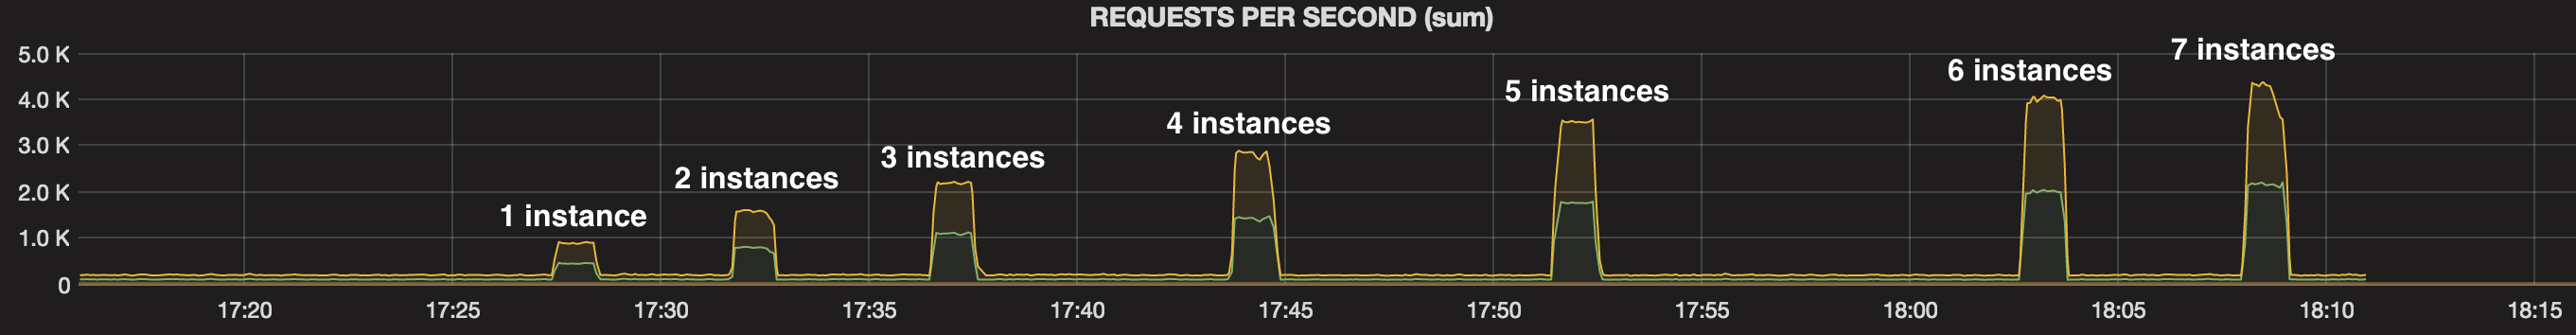
\includegraphics[width=14cm]{scale-load-generator}
	\caption{Load produced from different number of instances}
	\source{Grafana - Router Health}
	\label{scale-load-generator}
\end{figure}


A simple load generator is implemented in this project as a node application. It sends requests with unique correlation id in the header to the server, records the response time and stores them in database at the end of load generating. The application is deployed to cloud foundry and uses PostgreSQL backing service. A time-out mechanism is added to make sure load is generated in the given time frame. Except for producing fancy graphic analysis results, it pretty much accomplishes every thing a load generating tool can do. It is more flexible to work with raw data anyway.


\subsection{Features}
\label{load generator}
The majority of the load testing frameworks choose to generate a fixed number of total requests with given amount of concurrencies.  For example, a typical \textit{JMeter} test plan configures parameter \textit{Number of Threads} as concurrent virtual users. Through \textit{Loop Count}, the same concurrency is repeated so to reach the total number of requests. \textit{Hey} defines the total requests and concurrency degree then carry out the load generating accordingly. The same principle behind them is that the period of time during which the tests are carried out is not measured, only the response time of individual request. So many requests shall be sent either ended with successful transaction or landed in error because of timeout or other various reasons. \\
The load generator used in this project produces load in two ways. One implementation also generates the load with a fixed number of requests. Another implementation brings about parallel requests in a given fixed time frame, for example in one minute. The application will first pile up requests to a predefined parallel parameter. Whenever a request is successfully returned, a new one will be created to maintain the total parallel requests. Since the load testing is executed in an cloud environment where there are productive applications, define a relatively short time frame reduces influence on others. Therefore it is also used in the thesis most of the time. Figure \ref{load-generator} shows how load generator operates.\\
 \begin{figure}[h]
	\centering
	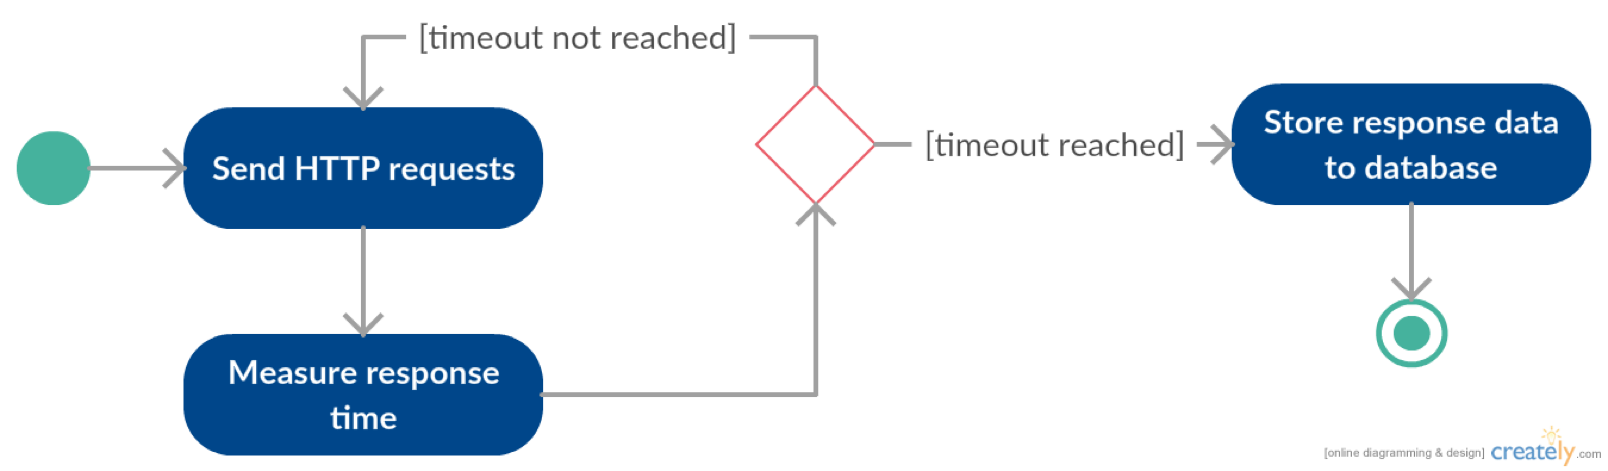
\includegraphics[width=10cm]{load-generator}
	\caption{Activity diagram of load generator}
	\label{load-generator}
\end{figure}
The proxy server limitation is discussed in \ref{haproxy}. At the beginning the requests on the server was always brought about through establishing new connections. This has quickly hit the limit of what the HAProxy can handle. To workaround it, the started connections are kept alive and reused. Although HAProxy has a strange setting of cutting off the connection after a period of time, when the time expanse of test is not set to this limit, all things work perfectly. 

\subsection{Limitations}
Since load generator is deployed as a worker in Cloud Foundry, it has little choice over database selection. In this project, a docker container version of database is used owing to the fact that other dedicated backing services are not free of charge. There are times container is simply overloaded and refuse to store any more data. \\
Secondly, load generator can be resource consuming as already discussed. In Cloud Foundry, some organization or space has only restricted size of memory to provide. It could be hard to scale the load generator to ideal capacity.In this thesis, for a period of time the load testing is conducted in a staging landscape of Cloud Foundry with a limited space quota of 10 G memory. Imagine all the applications and load generators scaling together, the space limit is easily exceeded. \\
Last but not the least, there is a chance the load generator is running on the same node as applications which will directly influence the CPU share the application could obtain and result in tainted test results. In the thesis, this unlucky scenario is avoided by deploying the load generator in DEA cells while the application is running in Diego cell. 

